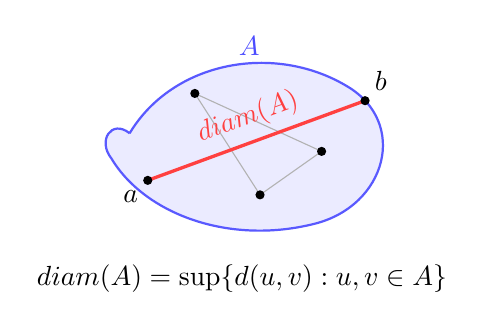
\begin{tikzpicture}[scale=0.92,>=stealth]
  \fill[blue!8]
    (0.0,0.0) .. controls (0.6,1.0) and (2.0,1.25) .. (3.0,0.65)
    .. controls (3.85,0.15) and (3.55,-1.0) .. (2.55,-1.25)
    .. controls (1.35,-1.55) and (0.2,-1.1) .. (-0.25,-0.35)
    .. controls (-0.45,-0.1) and (-0.25,0.2) .. (0.0,0.0);
  \draw[blue!65,thick]
    (0.0,0.0) .. controls (0.6,1.0) and (2.0,1.25) .. (3.0,0.65)
    .. controls (3.85,0.15) and (3.55,-1.0) .. (2.55,-1.25)
    .. controls (1.35,-1.55) and (0.2,-1.1) .. (-0.25,-0.35)
    .. controls (-0.45,-0.1) and (-0.25,0.2) .. (0.0,0.0);

  \coordinate (a) at (0.25,-0.65);
  \coordinate (b) at (3.25,0.45);
  \coordinate (c) at (0.9,0.55);
  \coordinate (d) at (1.8,-0.85);
  \coordinate (e) at (2.65,-0.25);

  \draw[gray!60] (c) -- (e);
  \draw[gray!60] (c) -- (d);
  \draw[gray!60] (d) -- (e);
  \draw[red!75,very thick] (a) -- (b)
    node[midway,above,sloped] {\(\operatorname{diam}(A)\)};

  \foreach \p/\lab/\pos in {a/a/below left,b/b/above right,c/{}/above,d/{}/below,e/{}/right}
  {
    \fill[black] (\p) circle (1.8pt);
    \node[\pos] at (\p) {\(\lab\)};
  }

  \node[blue!70] at (1.65,1.2) {\(A\)};
  \node[align=center] at (1.55,-2.0)
    {\(\operatorname{diam}(A)=\sup\{d(u,v):u,v\in A\}\)};
\end{tikzpicture}
